\documentclass[10pt,twocolumn,letterpaper]{article}

\usepackage{cite}
\usepackage{caption}
\usepackage{underscore}
\usepackage{cvpr}
\usepackage{times}
\usepackage{epsfig}
\usepackage{graphicx}
\usepackage{amsmath}
\usepackage{amssymb}
\usepackage[utf8]{inputenc}
\usepackage[T1]{fontenc}
\usepackage{lmodern} % load a font with all the characters

% Include other packages here, before hyperref.

% If you comment hyperref and then uncomment it, you should delete
% egpaper.aux before re-running latex.  (Or just hit 'q' on the first latex
% run, let it finish, and you should be clear).
\usepackage[breaklinks=true,bookmarks=false]{hyperref}

\cvprfinalcopy % *** Uncomment this line for the final submission

\def\cvprPaperID{****} % *** Enter the CVPR Paper ID here
\def\httilde{\mbox{\tt\raisebox{-.5ex}{\symbol{126}}}}

% Pages are numbered in submission mode, and unnumbered in camera-ready
%\ifcvprfinal\pagestyle{empty}\fi
\setcounter{page}{1}
\begin{document}

%%%%%%%%% TITLE
\title{Laboratorio 7: PHOW Classification}

\author{Rafael Cuperman Coifman\\
Universidad de los Andes\\
Bogotá, Colombia\\
{\tt\small r.cuperman675@uniandes.edu.co}
% For a paper whose authors are all at the same institution,
% omit the following lines up until the closing ``}''.
% Additional authors and addresses can be added with ``\and'',
% just like the second author.
% To save space, use either the email address or home page, not both
}

\maketitle
%\thispagestyle{empty}

%%%%%%%%% ABSTRACT
\begin{abstract}
La clasificación de imágenes de acuerdo a su contenido, es decir, el reconocimiento de objetos semánticamente dentro de imágenes, es un problema altamente atacado por varios investigadores en el área de la visión artificial. En este documento se presenta una aproximación a la solución a este problema mediante el uso de PHOW (una especie de descriptores SIFT a múltiples escalas) bajo la base de datos \textit{imagenet-tiny}, que contiene imágenes de difícil clasificación. Se varían tres parámetros para evaluar el desempeño y los recursos computacionales utilizados para entrenar y evaluar el modelo: cantidad de clases, número de imágenes de entrenamiento y partición espacial en X.
\end{abstract}

%%%%%%%%% BODY TEXT
%-------------------------------------------------------------------------
\section{Introducción}
Uno de los problemas de mayor envergadura en el área de la visión artificial es el reconocimiento de imágenes de acuerdo a su contenido. Existen varias técnicas para solucionarlo, por lo que los resultados y la base de las soluciones varían. En este trabajo se aborda el problema a partir del uso de descriptores SIFT, mediante \textit{bag of words}

\subsection{Base de datos \cite{vedaldi08vlfeat}} 
El problema de clasificación en este experimento se hace mediante el uso de la base de datos \textit{imagenet-tiny}, la cual está compuesta por imágenes divididas en 200 clases excluyentes de diverso tipo, tanto construcciones como seres vivos y elementos inertes. Al decir que las clases son excluyentes, se refiere a que cada imagen pertenece únicamente a una sola categoría.Cada clase tiene 100 imágenes a color con tamaño de 256x256 píxeles. Esta base de datos se considera una base de datos difícil de clasificar, ya que las imágenes dentro de cada categoría son muy variadas, encontrando situaciones de cambios del punto de vista, iluminación, escala, oclusión, deformación y variabilidad de apariencia entre cada clase. Estas características hacen que el problema sea más difícil de solucionar, ya que las imágenes están muy poco controladas al momento de capturarlas.

En la figura \ref{fig:ejemplos base de datos} se muestran ejemplos de imágenes de la base de datos. Nótese la diferencia de imágenes dentro de la misma clase, haciendo que la clasificación sea una tarea más compleja.

\begin{figure}[h]
    \centering
    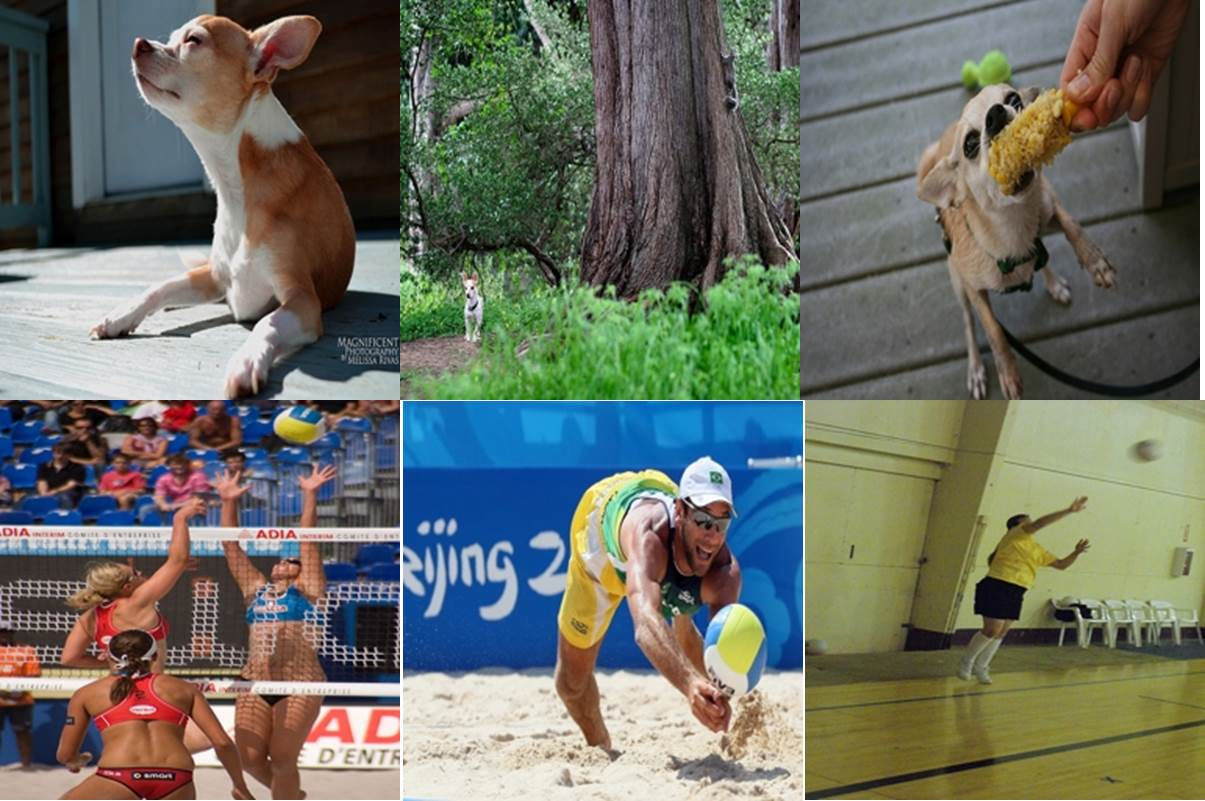
\includegraphics[width=0.5\textwidth]{EjemplosBaseDeDatos.jpg}
    \caption{Ejemplos de imágenes de la base de datos. Las tres imágenes superiores corresponden a la clase "Chihuahua"; las tres imágenes inferiores corresponden a la clase "Volleyball"}
    \label{fig:ejemplos base de datos}
\end{figure}

%------------------------------------------------------------------------
\section{Desarrollo}
El método de reconocimiento que se utilizó fue mediante descriptores PHOW, que son una variante de los descriptores densos SIFT (\textit{dense SIFT descriptors}). La función que permite hacer esto en Matlab fue bajada de \cite{vedaldi08vlfeat} y modificada levemente para poder ser utilizada sobre las imágenes de \textit{imagenet-tiny}. Las modificaciones realmente fueron pocas, ya que la misma función crea el diccionario de palabras para las imágenes de entrenamiento utilizadas. Se tuvo que modificar el formato de las imágenes a .JPEG para que la función las pueda encontrar y los nombres de las cases. Aparte de esto la función es suficientemente robusta para funcionar por si sola, tanto para entrenar con el SVM como para clasificar.

El método que se sigue es el siguiente: se obtienen algunos descriptores PHOW de las imágenes de entrenamiento para entrenar el diccionario, luego se clusterizan estas palabras con kmeans (600 clusters) para formar un diccionario de palabras (bag of words) de 600 de ellas. Este paso es sumamente importante, ya que con este se construye el diccionario a partir de las imágenes de entrenamiento y no a partir de otra base de datos. Luego de tener este pool de palabras, se encuentra la representación de las imágenes de entrenamiento mediante PHOW y la asociación a la bolsa de palabras ya construida anteriormente (encontrando a qué cluster de los 600 se encuentra más cercano). Con esto se tiene que cada imagen de entrenamiento se representa con un vector que determina la cantidad de "palabras visuales" que contiene del diccionario de 600 palabras. Esta representación de las imágenes de entrenamiento es la que se usa para entrenar un SVM, obteniendo el modelo de clasificador para las clases utilizadas. Finalmente, se evalúan las imágenes de test con este modelo hallando los scores y la matriz de confusión con su respectivo porcentaje de aciertos de clasificación. Este último paso requiere que cada imagen de test se represente como las imágenes de entrenamiento (descriptores PHOW seguidos de asociación de estos a la palabra visual \textit{bag of words} que corresponde. \cite{Szeliski}

Este procedimiento se realizó variando tres parámetros para evaluar el desempeño, tiempo y características del modelo en función de esos tres valores: número de clases, cantidad de imágenes de entrenamiento y partición espacial en X.
%-------------------------------------------------------------------------
\section{Resultados}
Los resultados de la clasificación de estas imágenes por medio de la metodología propuesta no son satisfactorios. Para todos los experimentos realizados, variando los diferentes parámetros, se encontraron porcentajes de clasificación correcta (de ahora en adelante llamada accuracy) bajos: alrededor del 30\% y 40\% casi siempre, hallando un máximo de 50\% al usar únicamente 5 clases, lo cual no es lo deseado.

El resultado del algoritmo planteado arroja dos gráficas, como se ve en la figura \ref{fig:resultado}:

La gráfica de la derecha corresponde a la matriz de confusión, donde color rojo corresponde a un nivel alto y azul a bajo. Lo ideal en este caso es tener la diagonal de la matriz completamente rojo y afuera de esta completamente azul. Los puntos que se encuentran fuera de la diagonal corresponden a clasificaciones erróneas, que contribuyen al error. Los dos ejes corresponden a las categorías.

La gráfica de la izquierda corresponde al \textit{score} que le otorga el clasificador a la clasificación de cada imagen evaluada. La escala de colores es igual que en la gráfica de la derecha. Cuando una imagen tiene un punto rojo oscuro en esta gráfica, quiere decir que el clasificador está muy seguro a cuál clase pertenece. El eje horizontal corresponde a cada una de las imágenes evaluadas y el eje vertical a las clases que pueden pertenecer. Esta gráfica muestra el resultado sobre las imágenes de entrenamiento y de evaluación con una diferenciación marcada. Como se puede observar en la gráfica de la izquierda de la figura \ref{fig:resultado}, hay una diagonal roja que va hasta 2000. Hasta ese punto se tienen las imágenes de entrenamiento, que son más fácilmente clasificadas correctamente, debido a que el modelo las usó para construirse. De las imágenes 2000 a 4000 se hallan puntos claros, casi siempre azules. Esto se debe a que esas imágenes son las de test, que no fueron vistas por el modelo y por lo tanto son más difíciles de clasificar correctamente. Con lo anterior se puede evidenciar un claro sobreajuste, ya que un buen clasificador debería poder clasificar igual de bien las imágenes de entrenamiento y de evaluación, con lo que se debería ver, en un modelo sin sobreajuste, una gráfica con dos diagonales oscuras como la que se observa hasta la imagen 2000 en la figura \ref{fig:resultado}.

\begin{figure}[h]
    \centering
    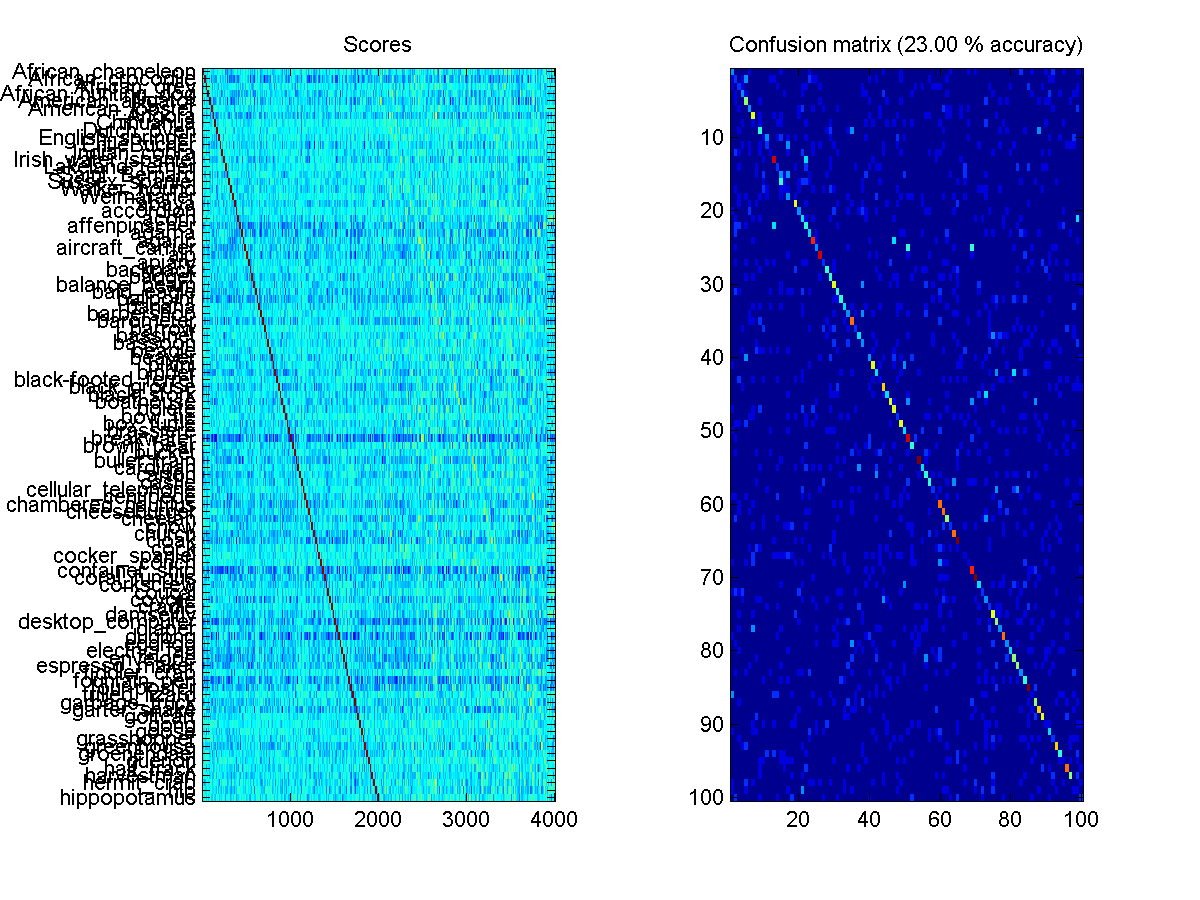
\includegraphics[width=0.5\textwidth]{Resultados.jpg}
    \caption{Ejemplo del resultado final del algoritmo de clasificación sobre imágenes. En este caso en específico se usaron 100 clases, 20 imágenes de entrenamiento y 20 imágenes de test por categoría}
    \label{fig:resultado}
\end{figure}

El trabajo se enfocó principalmente en ver el efecto de la variación de diferentes parámetros en el entrenamiento y clasificación de imágenes, más que en tratar de lograr un porcentaje de error bajo. Se midió el accuracy y el tiempo requerido para entrenar y clasificar las imágenes al variar tres parámetros importantes: número de categorías, número de imágenes de entrenamiento y número de particiones espaciales. Los resultados de accuracy se hicieron sobre las imágenes de test, ya que evaluar el desempeño sobre imágenes de entrenamiento no tiene sentido, ya que lo más probable es que se encuentre un nivel alto de \textit{overfitting} (sobreajuste). El verdadero desempeño se mide al evaluar imágenes que no fueron vistas en el proceso de entrenamiento, es decir, con las imágenes de test.

De acuerdo a o anterior, los resultados de accuracy al variar el número de clases, la cantidad de imágenes de entrenamiento y la partición espacial se encuentran en las figuras \ref{fig:clases}, \ref{fig:train} y \ref{fig:particion} respectivamente.

\begin{figure}[h]
    \centering
    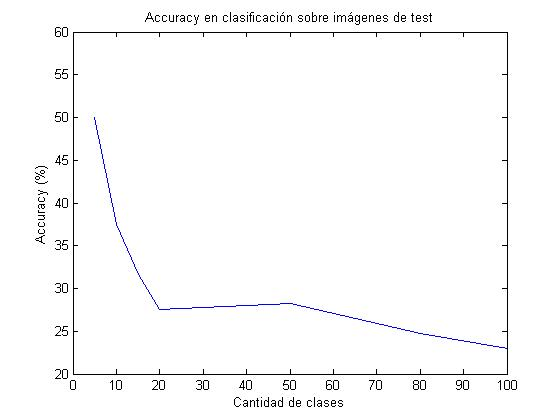
\includegraphics[width=0.5\textwidth]{VariacionNumClases.jpg}
    \caption{Desempeño de clasificación sobre imágenes de test al variar el número de clases. Para todos los casos se usaron 20 imágenes de entrenamiento, 20 imágenes de test por categoría y partición espacial (2,4)}
    \label{fig:clases}
\end{figure}

\begin{figure}[h]
    \centering
    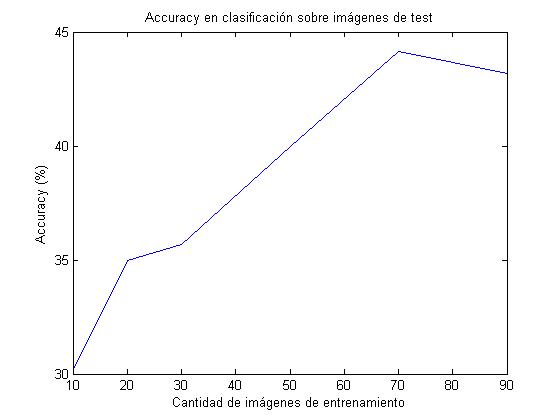
\includegraphics[width=0.5\textwidth]{VariacionNumTrain.jpg}
    \caption{Desempeño de clasificación sobre imágenes de test al variar el número de imágenes de entrenamiento. Para todos los casos se usaron 30 clases, 20 imágenes de test por categoría y partición espacial (2,1)}
    \label{fig:train}
\end{figure}

\begin{figure}[h]
    \centering
    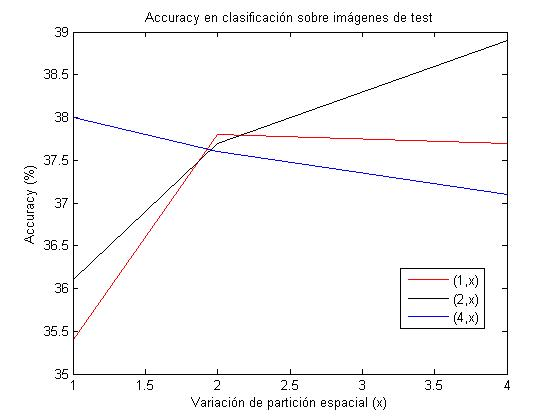
\includegraphics[width=0.5\textwidth]{VariacionNumSpatialX.jpg}
    \caption{Desempeño de clasificación sobre imágenes de test al variar la partición espacial. Para todos los casos se usaron 20 clases y 50 imágenes de entrenamiento y test por categoría}
    \label{fig:particion}
\end{figure}

La evaluación de recursos computacionales requeridos para cada caso se hizo midiendo el tiempo necesario para realizar cada uno de los entrenamientos y evaluaciones. Estos tiempos para la variación del número de clases, de la cantidad de imágenes de entrenamiento y de la partición espacial se encuentran en las figuras \ref{fig:tiempoclases}, \ref{fig:tiempotrain} y \ref{fig:tiempoparticion} respectivamente.

\begin{figure}[h]
    \centering
    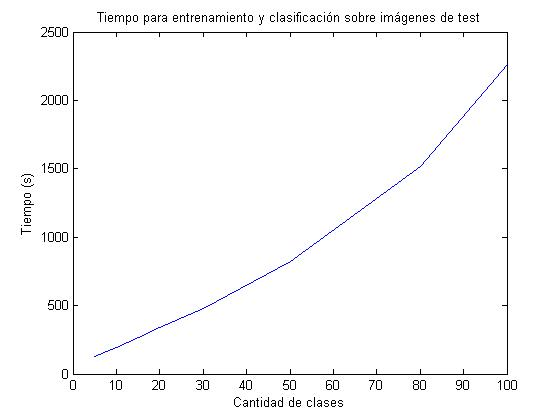
\includegraphics[width=0.5\textwidth]{TiempoVariacionNumClases.jpg}
    \caption{Tiempo requerido para entrenamiento y clasificación sobre imágenes de test al variar el número de clases. Para todos los casos se usaron 20 imágenes de entrenamiento, 20 imágenes de test por categoría y partición espacial (2,4)}
    \label{fig:tiempoclases}
\end{figure}

\begin{figure}[h]
    \centering
    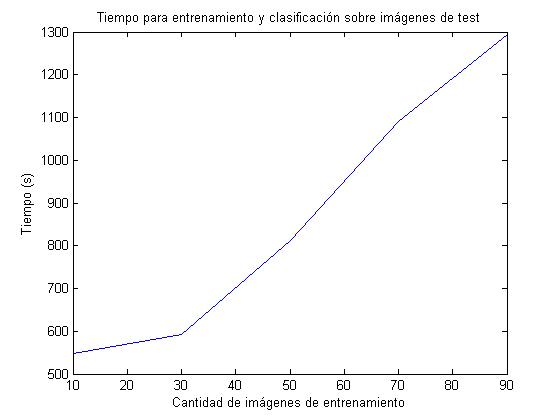
\includegraphics[width=0.5\textwidth]{TiempoVariacionNumTrain.jpg}
    \caption{Tiempo requerido para entrenamiento y clasificación sobre imágenes de test al variar el número de imágenes de entrenamiento. Para todos los casos se usaron 30 clases, 20 imágenes de test por categoría y partición espacial (2,1)}
    \label{fig:tiempotrain}
\end{figure}

\begin{figure}[h]
    \centering
    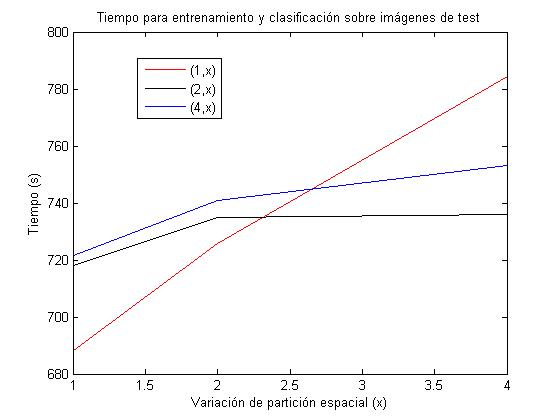
\includegraphics[width=0.5\textwidth]{TiempoVariacionNumSpatialX.jpg}
    \caption{Tiempo requerido para entrenamiento y clasificación sobre imágenes de test al variar la partición espacial. Para todos los casos se usaron 20 clases y 50 imágenes de entrenamiento y test por categoría}
    \label{fig:tiempoparticion}
\end{figure}

%-------------------------------------------------------------------------
\section{Discusión}
Los resultados de la clasificación de las imágenes de test no son satisfactorios en ningún caso de variación de los parámetros sobre esta base de datos. Esto se debe a que las imágenes de la base de datos son bastante complicadas de clasificar, debido a la variación que hay dentro de cada una de las categorías. Al hacer la clasificación sobre una base de datos más fácil (Caltech 101 \cite{Caltech}), es decir, con imágenes más uniformes y controladas, se encuentra un desempeño como el de la figura \ref{fig:caltech} (Accuracy de 68.5\%). En una base de datos más sencilla se ve en la matriz de \textit{scores} una segunda diagonal tenue, medio amarilla, para las imágenes de test, cosa que no se observa casi en la evaluación sobre una base de datos más complicada, como la usada en este documento.

\begin{figure}[h]
    \centering
    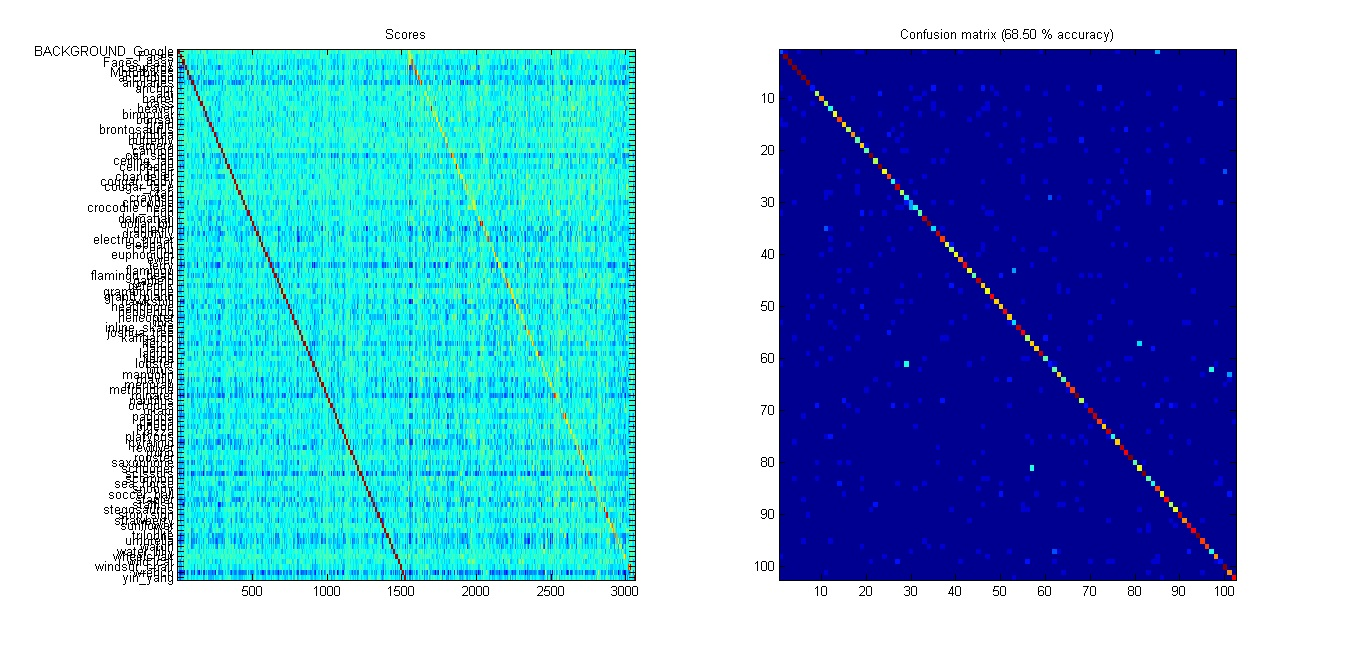
\includegraphics[width=0.5\textwidth]{ResultadosCaltech.jpg}
    \caption{Resultados de clasificación sobre imágenes de la base de datos Caltech101}
    \label{fig:caltech}
\end{figure}


Las gráficas presentadas muestran que hay una fuerte dependencia entre los parámetros usados (número de clases, cantidad de imágenes de train y partición espacial) en los recursos computacionales usados y en el desempeño de los clasificadores

\subsection{Variación del número de clases}
Al variar el número de clases, dejando constante los otros dos parámetros (cantidad de imágenes de entrenamiento y partición espacial), se tiene que construir un modelo más complejo, que incluye cada vez más categorías, a partir de la misma cantidad de imágenes de entrenamiento por clase. Esto se traduce en una disminución del desempeño de clasificación sobre imágenes de test, como se puede observar en la figura \ref{fig:clases}. A medida que aumenta el número de clases, el desempeño es peor, equivocándose más en la clasificación de imágenes. La relación no es lineal; más bien parece tener un comportamiento exponencial, mejorando el accuracy si se usan menos clases. Sin embargo, la idea de estos problemas es poder clasificar correctamente una gran cantidad de categorías, por lo que la solución no es usar menos de ellas sino modificar otros parámetros o el espacio de representación para lograr buenos resultados con una gran cantidad de clases. 

En cuanto al tiempo requerido para entrenar y evaluar al variar el número de clases, es intuitivo comprender que entre más categorías, el modelo es más complejo y por lo tanto se requiere mayor esfuerzo del computador para construir el clasificador. Esto se evidencia en la figura \ref{fig:tiempoclases}, donde a medida que se aumenta el número de clases, el tiempo requerido aumenta de manera casi lineal, haciendo que sea una situación altamente significativa.

\subsection{Variación de la cantidad de imágenes de entrenamiento usadas}
Al variar el número de imágenes de entrenamiento, dejando constante los otros dos parámetros (número de clases y partición espacial), se tienen más o menos imágenes para construir el modelo de la misma cantidad de categorías. Esto implica que entre más imágenes uno tenga para enseñarle al computador, este podrá aprender mejor una función clasificadora mejorando el desempeño. Una manera de ver esto es compararlo con el aprendizaje de un niño a matemáticas: entre más ejercicios se hagan, mejor va a aprender el niño. En la figura \ref{fig:train} se evidencia esto:a medida que aumenta el número de clases, el desempeño es mejor, equivocándose menos en la clasificación de imágenes hasta que se satura. La relación parece ser algo lineal; más bien parece tener un comportamiento exponencial, mejorando el accuracy si se usan más clases. De acuerdo a esto, en problemas de clasificación siempre se desea tener la mayor cantidad de imágenes de entrenamiento como sea posible.

En cuanto al tiempo requerido para entrenar y evaluar al variar el número de imágenes de entrenamiento entre más datos para enseñar, el computador requiere procesar más imágenes, haciendo un modelo más completo. Por lo tanto se requiere mayor esfuerzo de la máquina para construir el clasificador. Esto se evidencia en la figura \ref{fig:tiempotrain}, donde a medida que se aumenta el número de imágenes de entrenamiento, el tiempo requerido aumenta de manera casi lineal, haciendo que sea una situación significativa.

\subsection{Variación de la partición espacial}
La variación de este parámetro no es tan intuitivo como los otros. Este consta de un vector con dos números, por lo que se generaron tres gráficas: cada una correspondiente a la variación del segundo elemento del vector al dejar el primero fijo (para tres diferentes valores del primero vector). Con esto se evidencia que existe un valor para el primer número que tiende a ser más eficiente en el entrenamiento y clasificación. Cuando este primer valor fue 1, la variación de la segunda componente no tuvo una tendencia predecible, ya que por momentos aumentó y por otros disminuyó; cuando el primer valor fue 2, el aumento de la segunda dimensión generó un crecimiento en el accuracy; y cuando el primer número fue 4, el aumento del segundo valor provocó una disminución en el desempeño del clasificador. De acuerdo a esto, se puede llegar a pensar que es más provocativo utilizar el vector (2,4) para construir el modelo. 

En cuanto al tiempo requerido para entrenar y evaluar, se observó que en todos los casos, al aumentar el segundo número de este vector el tiempo aumentó, sin embargo, el crecimiento de esta gráfica fue completamente determinado por la primera dimensión de esta partición espacial. No sólo el accuracy del clasificador fue mejor usando (2,4), sino que el tiempo requerido fue menor también, esocogiendo este parámetro como el óptimo.
%-------------------------------------------------------------------------
\section{Conclusiones, limitaciones y posibles mejoras}
Al evaluar el desempeño de un clasificador basado en descriptores SIFT bajo la base de datos \textit{imagenet-tiny}, se encontró un desempeño mucho más bajo que el que se logró usando la base de datos \textit{Caltech 101}. Esto se debe a que las imágenes de la primera base de datos son mucho más complejas, teniendo problemas de oclusión, no rigidez y diferencias dentro de las clases, entre otras. Esta es una de las limitaciones del método utilizado, ya que en para Bag of Words se esperan que las palabras sean más rígidas, pero como estas imágenes son tan diferentes las unas a las otras, no se encuentran los mismos descriptores, perdiendo efectividad en la clasificación. Las imágenes de \textit{Caltech 101} son mucho más rígidas y estáticas, por lo cual se vio una mejor clasificación de las imágenes de test. 

Al variar los diferentes parámetros (número de clases, cantidad de imágenes de entrenamiento y partición espacial) dejando los otros fijos, se encuentra que el desempeño es altamente dependiente de estos. Al aumentar las clases pero mantener la misma cantidad de imágenes de entrenamiento, se disminuye el desempeño, ya que se debe construir un modelo más complejo usando la misma cantidad de datos. Por otro lado, se evidenció que entre más imágenes de entrenamiento se usen, mejor, debido a que para la misma cantidad de clases, entre más datos se tengan, el modelo puede llegar a ser más rico, generando un mejor clasificador. 

Una posible mejoría para lograr clasificar mejor estas imágenes de \textit{imagenet-tiny}, es tener en cuenta estas flexibilidades de los objetos, como por ejemplo modelándolos como partes unidas por resortes, lo cual permitiría una variación de la posición de las partes del objeto en el espacio de representación. Otra posibilidad es generar varios clasificadores dentro de las clases, para así permitir tener en cuenta la variación de las imágenes dentro de las categorías. Este enfoque se conoce como Exemplar SVM.

%-------------------------------------------------------------------------

{\small
\bibliographystyle{ieeetr}
\bibliography{bibliografia}
}

\end{document}